\documentclass[main.tex]{subfiles}

\begin{document}

\section{First and second law problems}

\subsection{~}
How much work is required to compress 5.00 moles of an ideal gas iso-thermally from 100 L to 40.0 L, at 300 K?

Knowing that is a reversible, iso-thermal process, the work can be computed as follows,
\begin{align*}
    W_{\mathrm{rev}} &= nRT\ln\qty[\frac{V_{o}}{V_f}] \\
    &= \SI{5}{\mol}\SI[per-mode=fraction]{8.314}{\joule\per\mole\per\kelvin}\SI{300}{\kelvin}\ln\qty[\frac{100}{40}],
\end{align*}
the total work is
\begin{gather*}
    \boxed{W = \SI{11.427}{\kilo\joule}}
\end{gather*}

%https://www.chegg.com/homework-help/questions-and-answers/calculate-minimum-amount-work-required-compress-500-moles-ideal-gas-isothermally-300-k-vol-q26947292

\subsection{~}
After 1.60 moles of NH3 gas is placed in a 1600 cm3 box at 25°C, the box is heated to 500 K. 
At this temperature, the ammonia is partially decomposed to N2 and H2 , and a pressure measurement gives 4.85 MPa. 
Find the number of moles of each component present at 500 K.
Notes: Assume the three components behave like ideal gases.
This partial decomposition of ammonia occurs according to the following stoichiometry:
$$2\mathrm{NH}_3\to \mathrm{N}_2+3\mathrm{H}_2$$

Assuming the ideal gas behavior, we can compute the number of $\mathrm{NH}_3$ moles at \SI{500}{\kelvin} assuming that no decomposition process occurs, as follows,
\begin{align*}
    PV &= nRT \\
    n &= \frac{PV}{RT} \\
    &= \frac{\SI{4.85d6}{\pascal}\SI{1.6d-3}{\meter\tothe{3}}}{\SI{8.314}{\pascal\meter\tothe{3}\per\kelvin\per\mol}\SI{500}{\kelvin}} \\
    &= \SI{1.867}{\mol},
\end{align*}

Now, we can find an equation that relates the number of moles of the N2 and H2 by taking into account the conservation of mass.
At the begging  of the process we get:
\begin{align*}
    2\mathrm{NH}_3 &\to \mathrm{N}_2 + 3\mathrm{H}_2 \\
    \SI{1.6}{\mol} &\to \SI{0}{\mol} + \SI{0}{\mol},
\end{align*}
at the end of the process we can state that,
\begin{align*}
    2\mathrm{NH}_3 &\to \mathrm{N}_2 + 3\mathrm{H}_2 \\
    -2x~\SI{}{\mol} &\to x~\SI{}{\mol} + 3x~\SI{}{\mol},
\end{align*}
adding both equations processes,
\begin{align*}
    1.60-2x \to x+3x.
\end{align*}
Now, taking into account the total number of moles previously computed using the ideal gas law,
\begin{align*}
    1.60-2x + x+3x &= \SI{1.867}{\mol}, \\
    x &= \SI{0.1335}{\mol}.
\end{align*}
Hence, the number of moles for each component are,
\begin{gather*}
    \boxed{\SI{1.333}{\mol}~\mathrm{of~NH}_3,} \\
    \boxed{\SI{0.1335}{\mol}~\mathrm{of~N}_2,} \\
    \boxed{\SI{0.4005}{\mol}~\mathrm{of~H}_2.}
\end{gather*}

%https://www.chegg.com/homework-help/questions-and-answers/q8068111?search=After%201.60%20mol%20of%20NH3%20gas%20is%20placed%20in%20a%201600-cm%5E3%20box%20at%2025%20degrees%20C%2C%20the%20box%20is%20heated%20to%20500%20K.%20At%20this%20temperature%2C%20the%20ammonia%20is%20partially%20decomposed%20to%20N2%20and%20H2%2C%20and%20a%20pressure%20measurement%20gives%204.85%20MPa.%20Find%20the%20number%20of%20moles%20of%20each%20component%20present%20at%20500%20K.&autotype=mix&typeaheadquestionid=q8068111&searchid=4b34e4d7-95e4-4325-a977-be494694a5fd&searchtype=typeahead&imagecounter=&fromSearch=true

\subsection{~}
One mole of He gas with $C_{V,m} = 3R/2$ essentially independent of temperature expands reversibly from \SI{24.6}{\liter} and \SI{300}{\kelvin} to \SI{49.2}{\liter}.
Calculate the final pressure and temperature if the expansion is
\begin{itemize}
    \item isothermal
    \item adiabatic
    \item Sketch these two processes on a P-V diagram
\end{itemize}

To compute the final pressure and temperature for each one of the systems and the relation pressure-volume for the diagram, we analyze the internal change of both systems and the ideal gas law.

\paragraph{Iso-thermal}~

The final temperature for this process is the same as the start of the process,
\begin{gather*}
    \boxed{\SI{300}{\kelvin}.}
\end{gather*}

To compute the final pressure we use the ideal gas law,
\begin{align*}
    P_fV_f &= nRT_f \\
    P_f &= \frac{\SI{1}{\mol}~\SI{8.314}{\joule\per\mol\per\kelvin}~\SI{300}{\kelvin}}{\SI{0.0492}{\meter\tothe{3}}},
\end{align*}
hence,
\begin{gather*}
    \boxed{P_f = \SI{50.695}{\kilo\pascal}}
\end{gather*}

\begin{comment}
For this process the change in internal energy is equal to zero ($\Delta U = q+W =0$), leading with the following characteristic,
\begin{gather*}
    W = -q.
\end{gather*}
Indicating that there is an heat exchange with the surroundings, allowing the iso-thermal process of the system.
To compute the work done by the gas during the expansion we integrate as follows,
\begin{align*}
    W_{\mathrm{rev}} &= -\int_{V_{1}}^{V_{2}} nRT\frac{1}{V}dV \\
    &= -nRT\ln\qty[\frac{V_{2}}{V_{1}}] \\
    &= -nRT\ln\qty[\frac{V_f}{V_o}] \\
    &= -\SI{1}{\mol}~\SI[per-mode=fraction]{8.314}{\joule\per\mole\per\kelvin}~\SI{300}{\kelvin}\ln\qty[\frac{49.2}{24.6}] \\
    &= -\SI{1728.847}{\joule}.
\end{align*}

Now to compute the final pressure we use the same relation of work as before and solve for the pressure,
\begin{align*}
    W &= \int_{V_o}^{V_f}-P dV \\
    &= -P\qty(V_f-V_o) \\
    P &= -\frac{W}{\qty(V_f-V_o)}.
\end{align*}
Replacing the expression for the work of the reversible process,
\begin{align*}
    P &= \frac{nRT\ln\qty[\frac{V_f}{V_o}]}{\qty(V_f-V_o)} \\
    &= \frac{\SI{1}{\mol}~\SI[per-mode=fraction]{8.314}{\joule\per\mole\per\kelvin}~\SI{300}{\kelvin}\ln\qty[\frac{49.2}{24.6}]}{\qty(\SI{0.0492}{\meter\tothe{3}}-\SI{0.0246}{\meter\tothe{3}})} \\
    &= \SI{70278.361}{\pascal}.
\end{align*}
\end{comment}

\paragraph{Adiabatic}~\label{par:adiabaticWork}

For an adiabatic process is important to acknowledge that for an adiabatic process the Boyle's law ($PV=\mathrm{cte}$) and Charles's law ($V/T=\mathrm{cte}$) does not applies.
So we need to take into account the following relations,
\begin{gather*}
    P_oV_o^\gamma = P_fV_f^\gamma, %\qquad T_oV_o^\gamma = T_fV_f^\gamma,
\end{gather*}
with $\gamma = 5/3$, because is an mono-atomic ideal gas.
Finally, to compute the final pressure and temperature we need to compute the initial pressure of the system using the ideal gas law.

\begin{align*}
    P_oV_o &= nRT_o \\
    P_o &= \frac{\SI{1}{\mol}~\SI{8.314}{\joule\per\mol\per\kelvin}~\SI{300}{\kelvin}}{\SI{0.0246}{\meter\tothe{3}}} \\
    &= \SI{101.390}{\kilo\pascal}.
\end{align*}

Now, for the final pressure we use the exponential relation,
\begin{align*}
    P_oV_o^\gamma &= P_fV_f^\gamma \\
    P_f &= P_o\qty(\frac{V_o}{V_f})^\gamma \\
    P_f &= \SI{101.390}{\kilo\pascal}\qty(\frac{24.6}{49.2})^{5/3},
\end{align*}
which gives,
\begin{gather*}
    \boxed{\SI{31.935}{\kilo\pascal}.}
\end{gather*}

Finally, for the final temperature we use the ideal gas law,
\begin{align*}
    PV &= nRT \\
    T &= \frac{PV}{nR} \\
    &= \frac{\SI{31.935}{\kilo\pascal}~\SI{0.0492}{\meter\tothe{3}}}{\SI{1}{\mol}~\SI{8.314}{\joule\per\mol\per\kelvin}},
\end{align*}
therefore,
\begin{gather*}
    \boxed{\SI{188.982}{\kelvin}}
\end{gather*}

\begin{comment}
\begin{align*}
    T_oV_o^\gamma &= T_fV_f^\gamma \\
    T_f &= T_o\qty(\frac{V_o}{V_f})^\gamma \\
    T_f &= \SI{300}{\kelvin}\qty(\frac{24.6}{49.2})^{5/3},
\end{align*}
which gives,
\begin{gather*}
    \boxed{\SI{94.494}{\kilo\pascal}.}
\end{gather*}
\end{comment}

\begin{comment}
In contrast with the iso-thermal process, there is no exchange of heat between the system and the surroundings, which means that there must be a change in temperature of the system.
Hence, the change in internal energy is equal to the work done by the expansion process.
Therefore, to compute the final pressure and temperature of the system, we need to known the work done by the gas in the adiabatic expansion process.

Also is important to acknowledge that for an adiabatic process the Boyle's law ($PV=\mathrm{cte}$) and Charles's law ($V/T=\mathrm{cte}$) does not applies.
So we need to take into account the following relations,
\begin{gather*}
    P_oV_o^\gamma = P_fV_f^\gamma,\qquad T_oV_o^\gamma = T_fV_f^\gamma,
\end{gather*}
with $\gamma = 5/3$, because is an mono-atomic ideal gas.

Now we can compute the work by a change in temperature of the system,
\begin{gather*}
    W = n C_v\qty(T_f-T_o),
\end{gather*}
and the final temperature with the previous relations of $V-T$,
\begin{align*}
    T_oV_o^{\gamma-1} &= T_fV_f^{\gamma-1} \\
    T_f &= T_o\qty(\frac{V_o}{V_f})^{\gamma-1}.
\end{align*}

With these relations, we can equate the change in temperature to a change in volume of the expansion and solve for the pressure,
\begin{align*}
    C_V\qty(T_f-T_o) &= -P\qty(V_f-V_o) \\
    P &= -C_V\frac{\qty(T_f-T_o)}{\qty(V_f-V_o)}.
\end{align*}
Replacing the expressions and values,
\begin{align*}
    P &= -C_V\frac{\qty(T_f-T_o)}{\qty(V_f-V_o)} \\
    &= -\frac{C_v T_o}{\qty(V_f-V_o)}\qty[\qty(\frac{V_o}{V_f})^{\gamma-1}-1] \\
    &= -\frac{\frac{3}{2}\SI{8.314}{\joule\per\mole\per\kelvin}~\SI{300}{\kelvin}}{\qty(\SI{0.0492}{\meter\tothe{3}}-\SI{0.0246}{\meter\tothe{3}})}\qty[\qty(\frac{24.6}{49.2})^{5/3-1}-1] \\
    &= \SI{55788.482}{\pascal}
\end{align*}

\end{comment}

\paragraph{Diagram}~

\begin{figure}[ht!]
    \centering
    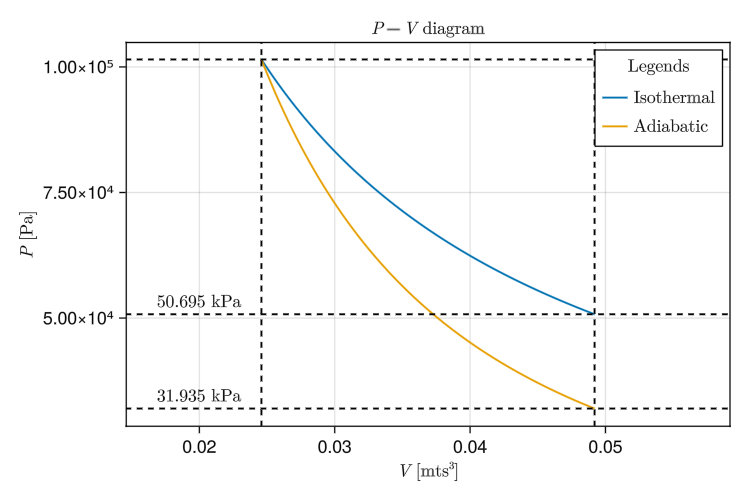
\includegraphics[width=0.9\linewidth]{imgs/hw2/pvDiagram.png}
    \caption{Comparison of the $P-V$ relation in an isothermal process with an adiabatic process.}
    %\label{fig:enter-label}
\end{figure}

\subsection{~}
For 2.00 g of Helium gas, find $q$, $w$, $\Delta U$, and $\Delta H$, if the gas undergoes:
\begin{itemize}
    \item a reversible constant-pressure expansion from \SI{20.0}{\deci\meter\tothe{3}} to \SI{40.0}{\deci\meter\tothe{3}}at 0.800 bar
    \item a reversible heating with P going from 0.600 bar to 0.900 bar while V remains fixed at \SI{15.0}{\deci\meter\tothe{3}}.
\end{itemize}

\paragraph{Isobaric expansion}~

First we convert the Helium gas grams to moles and the pressure from bar to Pascals,

\begin{minipage}[c]{\textwidth}
\begin{minipage}[c]{0.45\textwidth}
    \begin{gather*}
        \SI{0.800}{\bar} = \SI{0.800d5}{\pascal}
    \end{gather*}
\end{minipage}
\vrule
\begin{minipage}[c]{0.45\textwidth}
    \begin{align*}
        n &= \frac{m}{M} \\
        &= \frac{\SI{2.0}{\gram}}{\SI{4.00}{\gram\per\mol}} \\
        &= \SI{0.5}{mol},
    \end{align*}
\end{minipage}
\end{minipage}

Then, we compute the work done by the gas using the ideal gas law,
\begin{align*}
    w &= -P\qty(V_{f}-V_{o}) \\
    &= -\SI{0.800d5}{\pascal}\qty(\SI{4.0d-2}{\meter\tothe{3}}-\SI{2.0d-2}{\meter\tothe{3}}) \\
    &\begin{gathered}
        \boxed{w = -\SI{1.6}{\kilo\joule}.}
    \end{gathered}
\end{align*}

Now, to compute the heat transfer between the system and its surroundings at a constant pressure the following relation is used,
\begin{align*}
    q &= n C_{p,m}\Delta T.
\end{align*}
The heat capacity at constant pressure for Helium is $C_p = 5/2 R$, where $R=\SI{8.314}{\joule\per\mole\per\kelvin}$.
To compute the temperature difference,due to a change in volume, we use the ideal gas law as follows,
\begin{align*}
    \Delta T &= \frac{P}{nR}\qty(V_f - V_o) \\
    &= \frac{\SI{0.800d5}{\pascal}}{\SI{0.5}{\mol}\SI{8.314}{\joule\per\mole\per\kelvin}}\qty(\SI{4.0d-2}{\meter\tothe{3}}-\SI{2.0d-2}{\meter\tothe{3}}) \\
    &= \SI{384.892}{\kelvin}.
\end{align*}

Replacing the values of the variables to get the heat added to the system,
\begin{align*}
    q &= n C_p \Delta T \\
    &= \SI{0.5}{\mol}~\frac{5}{2}\SI[per-mode=fraction]{8.314}{\joule\per\mole\per\kelvin}\SI{384.892}{\kelvin} \\
    &\begin{gathered}
    \boxed{q = \SI{3.999}{\kilo\joule}}
    \end{gathered}
\end{align*}

For the change in internal energy we use the first law with the previous results,% the equation for ideal gas is used with $C_V = 3/2 R$,
\begin{align*}
    \Delta U &= q + W \\
    &= \SI{3.999}{\kilo\joule} - \SI{1.6}{\kilo\joule} \\
    &\begin{gathered}
        \boxed{\Delta U = \SI{2.399}{\kilo\joule}}
    \end{gathered}
\end{align*}

\paragraph{Isochoric expansion}~

In these process there is no work done due to the constant volume, so 
\begin{gather*}
    \boxed{w = \SI{0}{\joule}.}
\end{gather*}
To compute the heat exchange, we use the following relation with the ideal gas law,
\begin{align*}
    q_V &= nC_V\Delta T \\
    &= nC_V\frac{V}{nR}\qty(P_f-P_o) \\
    &= \SI{12.5}{\joule\per\mol\per\kelvin}\frac{\SI{15d-3}{\meter\tothe{3}}}{\SI{8.314}{\joule\per\mole\per\kelvin}}\qty(\SI{0.9d5}{\pascal}-\SI{0.6d5}{\pascal}) \\
    &\begin{gathered}
        \boxed{q_V = \SI{676.569}{\joule}}
    \end{gathered}
\end{align*}

For the change in internal energy we take into account the first law and the previous results,
\begin{align*}
    \Delta U &= q + W \\
    &= q \\
    &\begin{gathered}
        \boxed{\Delta U = \SI{676.569}{\joule}}
    \end{gathered}
\end{align*}

For the change in entalphy we consider the following equation,
\begin{align*}
    \Delta H &= \Delta U + P\Delta V + V\Delta P \\
    &= \Delta U + V\Delta P \\
    &= \SI{676.569}{\joule} + \SI{15d-3}{\meter\tothe{3}}\qty(\SI{0.9d5}{\pascal}-\SI{0.6d5}{\pascal}) \\
    &\begin{gathered}
        \boxed{\Delta H =\SI{1.126}{\kilo\joule}}
    \end{gathered}
\end{align*}

% https://www.chegg.com/homework-help/questions-and-answers/q108214025?search=Please%20show%20all%20work%20and%20explain%20it.%20Thank%20you%202%20%C2%A0mol%20of%20He%20gas%20with%20C_V%2C%20m%3D3%20R%20%2F%202%20expands%20reversibly%20from%205%20%C2%A0L%20and%20300%20%C2%A0K%20to%2015%20%C2%A0L.%20Treating%20H%20e%20as%20ideal%20gas%20calculate%20q%2C%20w%2C%20%5CDelta%20%20U%2C%20and%20final%20pressure%20and%20temperature%20if%20the%20expansion%20is%20(a)%20isothermal%3B%20(b)%20adiabatic.%20Hint%3A%20R%3D8.3145%20%C2%A0J%20%2F%20molK.&autotype=mix&typeaheadquestionid=q108214025&searchid=c3cdd4bc-c259-4195-84eb-1054f722b2cc&searchtype=typeahead&imagecounter=&fromSearch=true

% https://www.chegg.com/homework-help/questions-and-answers/q84313511?search=Type%20your%20answers%20in%20all%20of%20the%20blanks%20and%20submit%20Find%20q%2C%20w%2C%20%5CDelta%20%20U%2C%20and%2C%20%5CDelta%20%20H%20if%202.00%20g%20of%20helium%20gas%20undergoes%20a%20reversible%20constant-pressure%20expansion%20from%2020.0%20to%2040.0%20L%20at%200.800%20bar.%20q%3D%20w%3D%20k.%20%5B%20%5CDelta%20%20U%3D%3B%20%5CDelta%20%20H%3D%20%5D&autotype=mix&typeaheadquestionid=q84313511&searchid=04f9bd7c-cfc1-4609-8f29-499e1d830604&searchtype=typeahead&imagecounter=&fromSearch=true

\subsection{~}\label{subsec:5}
An ideal gas with, heat capacity ratio $\gamma = 1.40$, expands adiabatically. 
If the final temperature is one third of the initial one:
\begin{itemize}
    \item by what factor does the volume change?
    \item by what factor does the pressure change?
\end{itemize}

Knowing that is an adiabatic process, the relation between volume, pressure and temperature are modeled with the following equations,
\begin{gather*}
    P_oV_o^\gamma = P_fV_f^\gamma,\qquad T_oV_o^\gamma = T_fV_f^\gamma.
\end{gather*}

\paragraph{Volume change}~

Taking into account that $T_f = T_o/3$, the relation temperature-volume becomes,
\begin{align*}
    T_oV_o^\gamma &= \frac{1}{3}T_oV_f^\gamma \\
    V_o^\gamma &= \frac{1}{3}V_f^\gamma \\
    3^{1/\gamma}V_o &= V_f,
\end{align*}
indicating that the final volume expands $3^{1/\gamma}$ times with respect the original volume.
The difference in volume is,
\begin{align*}
    \Delta V &= 3^{1/\gamma}V_o - V_o \\
    &= V_o\qty(3^{1/\gamma} - 1) \\
    &= 1.191 V_o.
\end{align*}

\paragraph{Pressure change}~

Now that we know the volume change, we can compute the pressure change,
\begin{align*}
    P_oV_o^\gamma &= P_fV_f^\gamma \\
    P_oV_o^\gamma &= P_f\qty(3^{1/\gamma}V_o)^\gamma \\
    P_o &= 3P_f  \\
    \frac{1}{3}P_o &= P_f.
\end{align*}
Which is the same change as the temperature.
The difference is,
\begin{align*}
    \Delta P &= \frac{1}{3}P_o - P_o \\
    &= P_o\qty(\frac{1}{3}-1) \\
    &= -\frac{2}{3}P_o.
\end{align*}

\subsection{~}
Calculate the work involved when one mole of a monoatomic ideal gas at 198 K expands reversibly and adiabatically from a pressure of 10.00 bar to a pressure of 5.00 bar.

We follow a similar mathematical procedure of questions \ref{par:adiabaticWork} and \ref{subsec:5}.
In which we consider that no heat exchange between the system and the surroundings is done and the Boyles's and Charles's law does not applies.

The work is computed by the change in temperature of the system,
\begin{gather*}
    W = nC_V\qty(T_f-T_o).
\end{gather*}

The final temperature of the system can be computed as follows:
\begin{gather*}
    T_f = \qty(\frac{P_2}{P_1})^{R/C_{P,m}}T_o
\end{gather*}

Introducing this result into the work expression and replacing the variables with its numeric values,
\begin{align*}
    W &= nC_V\qty(\qty(\frac{P_2}{P_1})^{R/C_{P,m}}T_o-T_o) \\
    &= nC_V T_o\qty(\qty(\frac{P_2}{P_1})^{2/5}-1) \\
    &= \SI{1}{\mol}~\frac{3}{2}\SI[per-mode=fraction]{8.314}{\joule\per\mole\per\kelvin}~\SI{198}{\kelvin}\qty(\qty(\frac{5.00}{10.00})^{2/5}-1) \\
    &\begin{gathered}
        \boxed{W = -\SI{597.91}{\joule}.}
    \end{gathered}
\end{align*}

%www.chegg.com/homework-help/questions-and-answers/q149703976?search=Calculate%20the%20work%20involve%20when%20one%20mole%20of%20monoatomic%20ideal%20gas%20at%20298K%20expand%20reversibly%20and%20adiabatically%20from%20pressure%2010%20to%205%20bar.%20A.%20-900J%20B.%20900J%20C.%20934J&autotype=mix&typeaheadquestionid=q149703976&searchid=f0ffb6d5-bd1e-417a-8a12-898d29b3220f&searchtype=typeahead&imagecounter=&fromSearch=true

\subsection{~}
One mole of a monoatomic ideal gas is used as working fluid in a heat engine operating in a
reversible cycle ABCDA. 
At the initial point $A$, pressure, volume and temperature are $P_o , V_o $, and $T_o$ .
In point $B$, the pressure is $3P_o$ , and the volume is $V_o$. 
In point $C$, the pressure is $3P_o$ , and the volume is $2V_o$.
In point $D$, the pressure is $P_o$ , and the volume is $2V_o$.
In the process $A\to B$ an amount of heat $q_{1}$ is absorbed from the surroundings.
In process $B\to C$ an amount of heat $q_2$ is absorbed.
In process $C\to D$ an amount of heat $q_3$ is exchanged with the surroundings.
Finally, in process $D\to A$ an amount of heat $q_4$ is exchanged.

Draw a P-V diagram for this cycle and find the simplest expressions in terms of $R$ and $T_o$ for:
\begin{itemize}
    \item Total heat that enters the system in one cycle.
    \item Total heat that exits the system in one cycle.
 Using the results from the two questions above, calculate:   
    \item The efficiency of a heat engine that operates in this reversible cycle
    \item The efficiency of a Carnot engine that operates between the same minimum and maximum
temperatures
\end{itemize}

\begin{figure}[ht!]
    \centering
    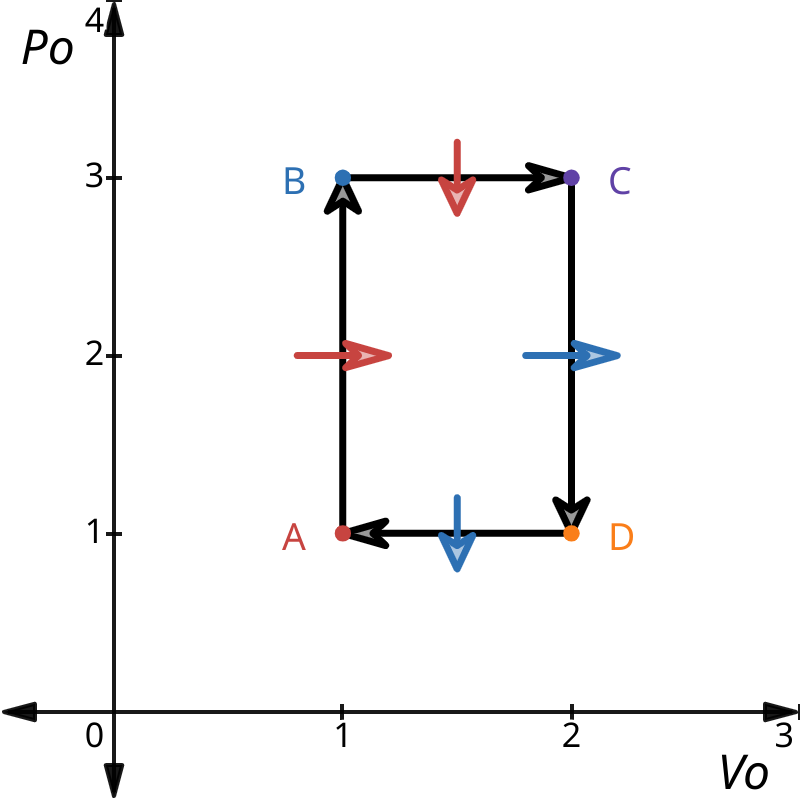
\includegraphics[width=0.45\linewidth]{imgs/hw2/cycle.png}
    \caption{Cycle of a heat engine. Red arrows indicate a heat transfer from the surroundings to the system and blue arrows indicate heat transfer from the system to the surroundings.}
    %\label{fig:enter-label}
\end{figure}

Taking into account that the cycle is composed of two isochoric and two isobaric processes, we can compute the heat exchange as follows,
\begin{align*}
    q_V &= nC_{V,m}\Delta T, \\
    q_P &= nC_{P,m}\Delta T.
\end{align*}

\paragraph{Total heat that enters the system.}~

The total heat entering the system occurs in the isochoric process $A\to B$ and in the isobaric process $B \to C$, hence, it can be computed as follows,
\begin{align*}
    q_{\mathrm{in}} &= q_{A\to B} + q_{B\to C} \\
    &= nC_{V,m}\Delta T_{A\to B} + nC_{P,m}\Delta T_{B\to C},
\end{align*}
the change in temperature between the points is computed using the ideal gas law,$T=PV/nR$,
\begin{align*}
    \Delta T_{A\to B} &= \frac{1}{nR}\qty(P_BV_B-P_AV_A), \\
    \Delta T_{B\to C} &= \frac{1}{nR}\qty(P_CV_C-P_BV_B),
\end{align*}
taking into account the relation given in the problem,
\begin{align*}
    \Delta T_{A\to B} &= \frac{1}{nR}\qty(3P_oV_o-P_oV_o) \\
    &= \frac{P_oV_o}{nR}\qty(3-1) \\
    &= 2\frac{P_oV_o}{nR}, \\
    \Delta T_{B\to C} &= \frac{1}{nR}\qty(3P_o2V_o-3P_oV_o) \\
    &= \frac{1}{nR}\qty(6P_oV_o-3P_oV_o) \\
    &= \frac{P_oV_o}{nR}\qty(6-3) \\
    &= 3\frac{P_oV_o}{nR},
\end{align*}
replacing this results into the heat relation,
\begin{align*}
    q_{\mathrm{in}} &= nC_{V,m}\Delta T_{A\to B} + nC_{P,m}\Delta T_{B\to C} \\
    &= nC_{V,m}2\frac{P_oV_o}{nR} + nC_{P,m}3\frac{P_oV_o}{nR} \\
    &= P_oV_o\qty(\frac{nC_{V,m}2}{nR} + \frac{nC_{P,m}3}{nR}) \\
    &= P_oV_o\qty(\frac{3}{2}\frac{R2}{R} + \frac{5}{2}\frac{R3}{R}) \\
    &= P_oV_o\qty(\frac{3}{2}2 + \frac{5}{2}3) \\
    &\begin{gathered}
        \boxed{q_{\mathrm{in}} =  10.5nRT_o}
    \end{gathered}
\end{align*}

\paragraph{Total heat that exit the system}~

To compute the heat transfer from the system to its surroundings we use a similar process as before, but taking into account that the process from $C\to D$ is isochoric and the process from $D\to A$ is isobaric.
\begin{align*}
    q_{\mathrm{out}} &= q_{C\to D} + q_{D\to A} \\
    &= nC_{V,m}\Delta T_{C\to D} + nC_{P,m}\Delta T_{D\to A},
\end{align*}
the change in temperature between the points is computed using the ideal gas law,$T=PV/nR$,
\begin{align*}
    \Delta T_{C\to D} &= \frac{1}{nR}\qty(P_o2V_o-3P_o2V_o) \\
    &= \frac{P_oV_o}{nR}\qty(2-6) \\
    &= -4\frac{P_oV_o}{nR}, \\
    \Delta T_{D\to A} &= \frac{1}{nR}\qty(P_oV_o-P_o2V_o) \\
    &= \frac{P_oV_o}{nR}\qty(1-2) \\
    &= -\frac{P_oV_o}{nR},
\end{align*}
replacing the results,
\begin{align*}
    q_{\mathrm{out}} &= nC_{V,m}\Delta T_{C\to D} + nC_{P,m}\Delta T_{D\to A} \\
    &= nC_{V,m}\qty(-4\frac{P_oV_o}{nR}) + nC_{P,m}\qty(-\frac{P_oV_o}{nR}) \\
    &= -P_oV_o\qty(4\frac{nC_{V,m}}{nR} + \frac{nC_{P,m}}{nR}) \\
    &= -P_oV_o\qty(4\frac{3}{2}\frac{R}{R} + \frac{5}{2}\frac{R}{R}) \\
    &= -P_oV_o\qty(4\frac{3}{2} + \frac{5}{2}) \\
    &\begin{gathered}
        \boxed{q_{\mathrm{out}} = -8.5nRT_o}
    \end{gathered}
\end{align*}

\paragraph{Efficiency of the heat engine}~

To compute the efficiency we use the following equation,
\begin{gather*}
    e = \frac{w}{q_{\mathrm{in}}},
\end{gather*}
and for a cyle, the work can be computed as follows,
\begin{align*}
    w &= q_{\mathrm{in}} + q_{\mathrm{out}} \\
    &= 10.5P_oV_o - 8.5P_oV_o \\
    &= 2P_oV_o,
\end{align*}
replacing that value into the efficiency relation,
\begin{align*}
    e &= \frac{2P_oV_o}{10.5P_oV_o} \\
    &\begin{gathered}
        \boxed{e = 0.1904}
    \end{gathered}
\end{align*}

\paragraph{Carnot efficiency}~

For the carnot efficiency we use the following equation,
\begin{gather*}
    e_{\mathrm{carnot}} = 1-\frac{T_c}{T_h}.
\end{gather*}
Where $T_c = T_o$ and $T_h$ is computed by the ideal gas law in point $C$,
\begin{align*}
    T_C & = \frac{3P_o2V_o}{nR} \\
    &= 6\cancelto{T_o}{\frac{P_oV_o}{nR}} \\
    &= 6T_o.
\end{align*}
Replacing in the Carnot efficiency expression,
\begin{align*}
    e_{\mathrm{carnot}} &= 1-\frac{T_o}{6T_o} \\
    &\begin{gathered}
        \boxed{e_{\mathrm{carnot}} = 0.8333.}
    \end{gathered}
\end{align*}

% https://www.chegg.com/homework-help/questions-and-answers/q83739741?search=2.%20(10%20points)%20One%20mole%20of%20a%20monoatomic%2C%20ideal%20gas%20goes%20through%20the%20cycle%20shown%20in%20the%20diagram.%20Paths%20AB%20and%20CD%20are%20adiabatic%2C%20while%20paths%20BC%20and%20DA%20are%20isobaric.%20Find%20T4%2C%20T5%2C%20Tc%2C%20and%20To%20P%20P%202PO%20-%20%D1%81%20adiab.%20adiabatic%20P.%20V.%202v.&autotype=mix&typeaheadquestionid=q83739741&searchid=2dc14936-dbd2-4d1d-9d48-5c7d52dd73ca&searchtype=typeahead&imagecounter=&fromSearch=true

\subsection{~}
Calculate $\Delta U, \Delta H$ and $\Delta S$ for each of the following changes in state of 2.50 mol of an ideal monoatomic gas with $C_{V,m} 1.5R$ (constant for all temperatures):
\begin{itemize}
    \item (1.50 atm, 400 K) → (3.00 atm, 600 K)
    \item (2.50 atm, 20.0 L) → (2.00 atm, 30.0 L)
    \item (28.5 L, 400 K) → (42.0 L, 400 K).
\end{itemize}

It is important to remember that $C_{P,m}-C_{V,m} = R$, which leads to $C_{P,m} = 5/2 R$.

\paragraph{Pressure and temperature change}~

In these processes, we assume a constant volume; therefore, no work is equal to zero, and the change of internal energy is equal to the heat transfer owing to the change in temperature.
Hence, the change in internal energy can be computed as follows,
\begin{align*}
    \Delta U &= q \\
    &= nC_{V,m}\Delta T \\
    &= \SI{2.50}{\mol}~\frac{3}{2}\SI[per-mode=fraction]{8.314}{\joule\per\mole\per\kelvin}\qty(\SI{600}{\kelvin}-\SI{400}{\kelvin}) \\
    &\begin{gathered}
        \boxed{\Delta U = \SI{6235.5}{\joule}.}
    \end{gathered}
\end{align*}

For the change in entropy can be computed using the relation of the ideal gas law,
\begin{align*}
    \Delta H &= nC_{P,m}\Delta T \\
    &= \SI{2.5}{\mol}\frac{5}{2}\SI{8.314}{\joule\per\mol\per\kelvin}\qty(\SI{600}{\kelvin}-\SI{400}{\kelvin}) \\
    &\begin{gathered}
        \boxed{\Delta H = \SI{10.392}{\kilo\joule}.}
    \end{gathered}
\end{align*}

Then, for the change in entropy,
\begin{align*}
    \Delta S &= n C_P\ln\qty(\frac{T_f}{T_o}) + n R \ln\qty(\frac{P_o}{P_f}) \\ 
    &= \SI{2.5}{mol}1.5\SI{8.314}{\joule\per\mole\per\kelvin}\ln\qty(\frac{600}{400}) + \SI{2.5}{\mol}\SI{8.314}{\joule\per\mole\per\kelvin}\ln\qty(\frac{1.5}{3}) \\
    &\begin{gathered}
        \boxed{\Delta S = \SI{6.6}{\joule\per\kelvin}}
    \end{gathered}
\end{align*}

\paragraph{Pressure and volume change}~

Using the same equations as before, we can compute the change in internal energy, entalpy and entropy.
The change in temperature is computed using the ideal gas law.
\begin{align*}
    T &= \frac{PV}{nR} \\
    \rightarrow & \Delta T = \frac{1}{nR}\qty(P_fV_f - P_oV_o).
\end{align*}

Replacing the expression for the change in temperature,
\begin{align*}
    \Delta U &= q \\
    &= nC_{V,m}\frac{1}{nR}\qty(P_fV_f - P_oV_o) \\
    &= n\frac{3}{2}R\frac{1}{nR}\qty(P_fV_f - P_oV_o) \\
    &= \frac{3}{2}\qty(P_fV_f - P_oV_o) \\
    &= \frac{3}{2}\qty(\SI{202650}{\pascal}~\SI{0.03}{\meter\tothe{3}} - \SI{253312.5}{\pascal}~\SI{0.02}{\meter\tothe{3}}) \\
    &\begin{gathered}
        \boxed{\Delta U = \SI{1.519}{\kilo\joule}.}
    \end{gathered}
\end{align*}

For the change in entropy the expression is,
\begin{align*}
    \Delta H &= nC_{P,m}\Delta T \\
    &=  n\frac{5}{2}R\frac{1}{nR}\qty(P_fV_f - P_oV_o) \\
    &=  \frac{5}{2}\qty(P_fV_f - P_oV_o) \\
    &= \frac{5}{2}\qty(\SI{202650}{\pascal}~\SI{0.03}{\meter\tothe{3}} - \SI{253312.5}{\pascal}~\SI{0.02}{\meter\tothe{3}}) \\
    &\begin{gathered}
        \boxed{\Delta H = \SI{2.533}{\kilo\joule}.}
    \end{gathered}
    %&= \SI{2.5}{\mol}\frac{5}{2}\SI{8.314}{\joule\per\mol\per\kelvin}\qty(\SI{600}{\kelvin}-\SI{400}{\kelvin}) \\
    %&\begin{gathered}
    %    \boxed{\Delta H = \SI{10.392}{\kilo\joule}.}
    %\end{gathered}
\end{align*}


The change in entropy for this process is computed as follows,
\begin{align*}
    \Delta S &= n C_V\ln\qty(\frac{T_f}{T_o}) + n R \ln\qty(\frac{V_f}{V_o}) \\ 
    &= n C_V\ln\qty(\frac{P_fV_f}{nR}\frac{nR}{P_oV_o}) + n R \ln\qty(\frac{V_f}{V_o}) \\
    &= n C_V\ln\qty(\frac{P_fV_f}{P_oV_o}) + n R \ln\qty(\frac{V_f}{V_o}) \\ 
    &= \SI{2.5}{mol}\frac{3}{2}~\SI{8.314}{\joule\per\mole\per\kelvin}\ln\qty(\frac{2\cdot30}{2.5\cdot20}) + \SI{2.5}{mol}~\SI{8.314}{\joule\per\mole\per\kelvin}\ln\qty(\frac{30}{20}) \\
    &\begin{gathered}
        \boxed{\Delta S = \SI{14.1}{\joule\per\kelvin}.}
    \end{gathered}
\end{align*}


\paragraph{Expansion at constant temperature}~

If the process is completed with constant temperature, the change is zero, which leads to,
\begin{gather*}
    \boxed{\Delta U = 0,} \\
    \boxed{\Delta H  = 0.}
\end{gather*}

finally, for the change in entropy,
\begin{align*}
    \Delta S &= nR\ln\qty(\frac{V_f}{V_o}) \\ 
    &= \SI{2.50}{\mol}~\SI[per-mode=fraction]{8.314}{\joule\per\mole\per\kelvin}\ln\qty(\frac{42.0}{28.5}) \\
    &\begin{gathered}
        \boxed{\Delta S = \SI{8.059}{\joule\per\kelvin}}
    \end{gathered}
\end{align*}


% https://www.chegg.com/homework-help/questions-and-answers/q125882082?search=Calculate%20Delta%20S%20for%20each%20of%20the%20following%20changes%20in%20state%20of%202.50%20mol%20of%20a%20perfect%20monatomicgas%20(ideal%20gas)%20with%20Cv%2Cm%20%3D1.5R%20for%20all%20temperatures%3A%20(a)%20(1.50%20atm%2C%20400%20K)%20(3.00%20atm%2C600%20K)%3B%20(b)%20(2.50%20atm%2C%2020.0%20L)%20(2.00%20atm%2C%2030.0%20L).&autotype=mix&typeaheadquestionid=q125882082&searchid=182393f8-039d-495d-a624-cbd62e0aec1b&searchtype=typeahead&imagecounter=&fromSearch=true

\subsection{~}
Calculate the entropy change when mixing two moles of nitrogen gas and 1 mole of oxygen gas, at the same temperature and pressure, assuming ideal behavior.

The change in entropy can be computed with the following equation,
\begin{align*}
    \Delta S &= -n_a R \ln\qty(x_a) -n_b R \ln\qty(x_b)  \\
    &= -\SI{2}{\mol}~\SI{8.314}{\joule\per\mol\per\kelvin}\ln\qty(\frac{2}{3}) -\SI{1}{\mol}~\SI{8.314}{\joule\per\mol\per\kelvin}\ln\qty(\frac{1}{3}) \\
    &\begin{gathered}
        \boxed{\Delta S = \SI{15.875}{\joule\per\kelvin}}
    \end{gathered}
\end{align*}

% https://www.chegg.com/homework-help/questions-and-answers/q114710167?search=Determine%20the%20entropy%20change%20when%20a%202.5%20g%20smaple%20of%20oxygen%20gas%20is%20mixed%20with%204.3%20grams%20of%20nitrogen.%205)%20(2%20points)%20Determine%20the%20entropy%20change%20when%20a%202.5%20%C2%A0g%20sample%20of%20oxygen%20gas%20is%20mixed%20with%204.3%20grams%20of%20nitrogen%20gas.&autotype=mix&typeaheadquestionid=q114710167&searchid=bac87529-6ef1-459c-a286-a0def6fb1aa8&searchtype=typeahead&imagecounter=&fromSearch=true

% https://www.chegg.com/homework-help/questions-and-answers/q114710167?search=Determine%20the%20entropy%20change%20when%20a%202.5%20g%20smaple%20of%20oxygen%20gas%20is%20mixed%20with%204.3%20grams%20of%20nitrogen.%205)%20(2%20points)%20Determine%20the%20entropy%20change%20when%20a%202.5%20%C2%A0g%20sample%20of%20oxygen%20gas%20is%20mixed%20with%204.3%20grams%20of%20nitrogen%20gas.&autotype=mix&typeaheadquestionid=q114710167&searchid=bac87529-6ef1-459c-a286-a0def6fb1aa8&searchtype=typeahead&imagecounter=&fromSearch=true

\end{document}